\subsection{Glyph: \glyph{Association}}
\label{sec:association}

The \glyph{association} between one or more \glyph{EPNs} represents the non-covalent binding of the biological entities represented by those \glyph{EPNs} into a larger complex.

\begin{glyphDescription}

\glyphSboTerm
SBO:0000177 ! non-covalent binding

\glyphIncoming
One or more \glyph{consumption} arcs (\sect{consumption}), zero or more \glyph{modulation} arcs (\sect{modulations}).

\glyphOutgoing
One \glyph{production} arc (\sect{production}).

\glyphContainer
An \glyph{association} is represented by a circular filled shape.
The shape is linked to two ports, that are small arcs attached to the centres of opposite sides of the shape, as shown in \fig{association}.
The incoming \glyph{consumption} (\sect{consumption}) and outgoing \glyph{production} (\sect{production}) arcs are linked to the extremities of those ports.

The \glyph{modulation arcs} (\sect{modulations}) point to the other two sides of the shape.

\glyphLabel
None.

\glyphAux
None.

\end{glyphDescription}

\begin{figure}[H]
  \centering
  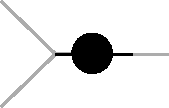
\includegraphics{images/build/association.pdf}
  \caption{The \PD glyph for \glyph{association}.}
  \label{fig:association}
\end{figure}

The example in \fig{assoc-cyclin} illustrates the association of cyclin and CDC2 kinase into the Maturation Promoting Factor.

\begin{figure}[H]
  \centering
  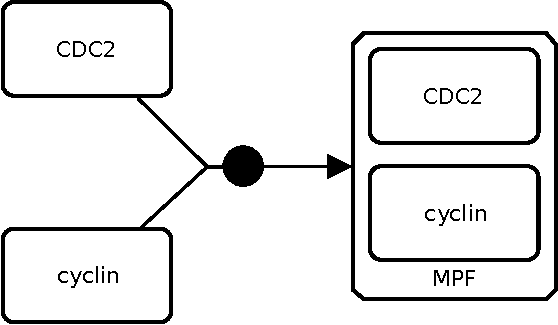
\includegraphics[scale = 0.8]{images/build/association_mpf_example.pdf}
  \caption{Association of cyclin and CDC2 kinase into the Maturation Promoting Factor.}
  \label{fig:assoc-cyclin}
\end{figure}

\fig{assoc-unamed} gives an example illustrating the association of a pentameric macromolecule (a nicotinic acetylcholine receptor) with a simple chemical (the local anesthetic chlorpromazin) in an unnamed complex.

\begin{figure}[H]
  \centering
  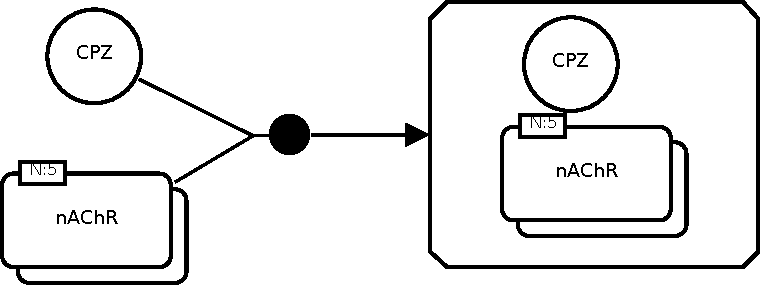
\includegraphics[scale = 0.8]{images/build/association_unamed_example.pdf}
  \caption{The association of a pentameric macromolecule with a simple chemical in an unnamed complex.}
  \label{fig:assoc-unamed}
\end{figure}

An association does not necessarily result in the formation of a \glyph{complex}; it can also produce a \glyph{multimer}, or a \glyph{macromolecule} (although the latter case is semantically borderline).  \fig{assoc-multi} gives an example of this, using the formation of hemoglobin.

\begin{figure}[H]
  \centering
  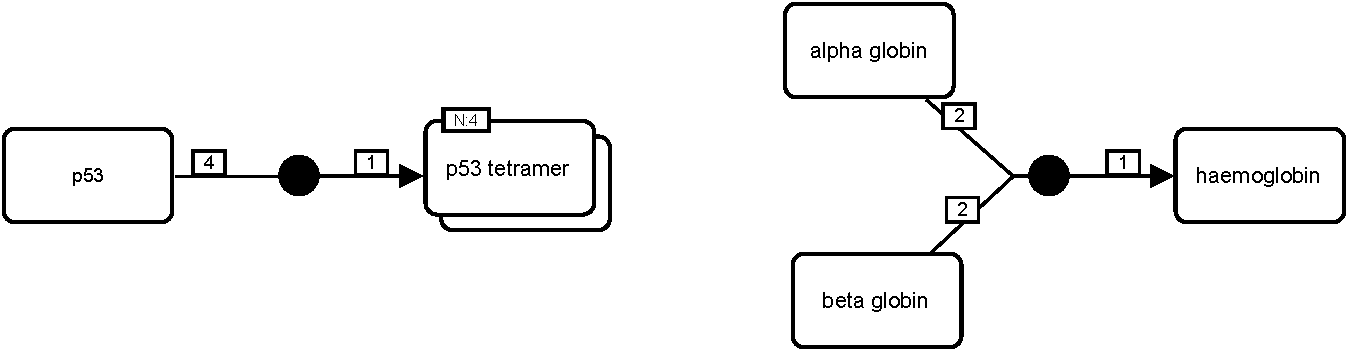
\includegraphics[scale = 0.8]{images/build/association_multimerisation_example.pdf}
  \caption{Formation of hemoglobin.}
  \label{fig:assoc-multi}
\end{figure}
